\section{Problem definition}

\begin{frame}[plain]
   \sectionpage
\end{frame}

\begin{frame}
   \frametitle{Our target problem}

   \textbf{Seeking for a \emph{core} optimization problem}
   \begin{itemize}
%      \item No standard instance dataset \citep{fikar2017, grenouilleau2020}
      \item Complex ``enough''
      \item Not too much constrained/specific
   \end{itemize}

   \vspace*{12pt}

   \textbf{The home health care routing and scheduling problem}
   \begin{itemize}
      \item HHCRSP was introduced by \citet{mankowska2014}
      \item Routing (caregivers) and scheduling (visit time)
      \item A model, and heuristics
      \item A public standard benchmark dataset
   \end{itemize}

%   \vspace{20pt}

%   \centering\includegraphics[width=0.9\textwidth]{img/skilled}

\end{frame}

\frame{
   \frametitle{The HHCRSP}

   \textbf{Main characteristics}
   \begin{enumerate}
      \item Routing components
      \item Patient time-window
      \item Covered service types
      \item Operations synchronization on multiple visits
   \end{enumerate}
}

\frame{
   \frametitle{The HHCRSP}

   \textbf{Main characteristics}
   \begin{enumerate}
      \item \textcolor{InfRed}{Routing components}
      \item Patient time-window
      \item Covered service types
      \item Operations synchronization on multiple visits
   \end{enumerate}
}

\frame{
   \frametitle{The HHCRSP: Routing features}
   \textbf{Routing components}
   \begin{itemize}
      \item Single transportation mode
      \item Routes start and finish at the depot
      \item Travel time between locations
      \item All visits must be performed
   \end{itemize}

%   \vspace*{12pt}

   \begin{figure}
      \includegraphics[width=0.9\textwidth,page=7]{fig/routing-example}
   \end{figure}
}

\frame{
   \frametitle{The HHCRSP}

   \textbf{Main characteristics}
   \begin{enumerate}
      \item \onlyh{1}{InfRed}{Routing components}
      \item \onlyh{2}{InfRed}{Patient time-window}
      \item Covered service types
      \item Operations synchronization on multiple visits
   \end{enumerate}
}

\frame{
   \frametitle{The HHCRSP: Routing features}
   \textbf{Soft time-window}
   \begin{itemize}
      \item Each patient/node has a time-window
      \item ``Hard'' time-window start
      \item ``Soft'' time-window ending
      \item Violated time-window ending: incurs additional cost
   \end{itemize}

   \begin{figure}[H]
      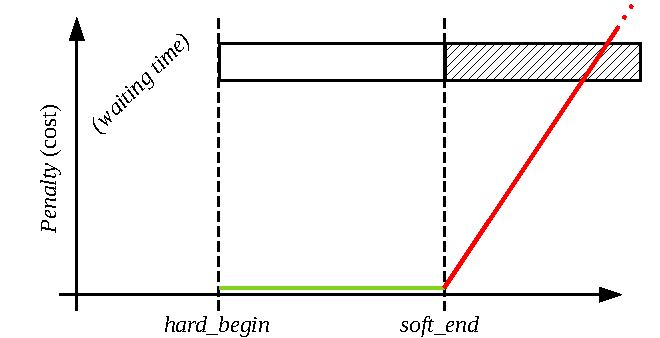
\includegraphics[width=0.7\textwidth]{fig/tw-penal.pdf}
   \end{figure}
}

\frame{
   \frametitle{The HHCRSP}

   \textbf{Main characteristics}
   \begin{enumerate}
      \item Routing components
      \item \onlyh{1}{InfRed}{Patient time-window}
      \item \onlyh{2}{InfRed}{Covered service types}
      \item Operations synchronization on multiple visits
   \end{enumerate}
}

\frame{
   \frametitle{The HHCRSP: domain features}

   \textbf{Covered service types}
   \begin{itemize}
      \item Set $\Sk$ of offered services
      \item A patient can require \textit{one}, or \textit{two services}
      \item Each service requested has a \textit{processing time}
      \item Caregivers have \textit{qualification} to perform only a few service types
   \end{itemize}

   \vspace*{8pt}

    \begin{figure}[H]
      \includegraphics[width=0.9\textwidth]{fig/skilled}
   \end{figure}

}

\frame{
   \frametitle{The HHCRSP}

   \textbf{Main characteristics}
   \begin{enumerate}
      \item Routing components
      \item Patient time-window
      \item \onlyh{1}{InfRed}{Covered service types}
      \item \onlyh{2}{InfRed}{Operations synchronization on multiple visits}
   \end{enumerate}
}


\begin{frame}
   \frametitle{The HHCRSP: domain features}
   \textbf{Operations synchronization on double service patients}
   \begin{itemize}
      \item Special requirement for patients requiring two service types
      \item Services must start simultaneously in some patients
      \item Others have precedence constraints
      \item Common feature container allocation/transshipment problems \citep{drexl2012synchronization}
   \end{itemize}

%   \vspace*{8pt}

   \begin{figure}[H]
      \includegraphics[width=1\textwidth,page=2]{fig/skilled}
   \end{figure}

\end{frame}

\begin{frame}
   \frametitle{The HHCRSP: Own characteristics}
   \textbf{Double service: precedence order}
   \begin{itemize}
      \item Service precedence: 2 > 5
      \item ($\delta^\mathrm{min}$) and ($\delta^\mathrm{max}$): separation time
   \end{itemize}

   \begin{figure}
      \centering
      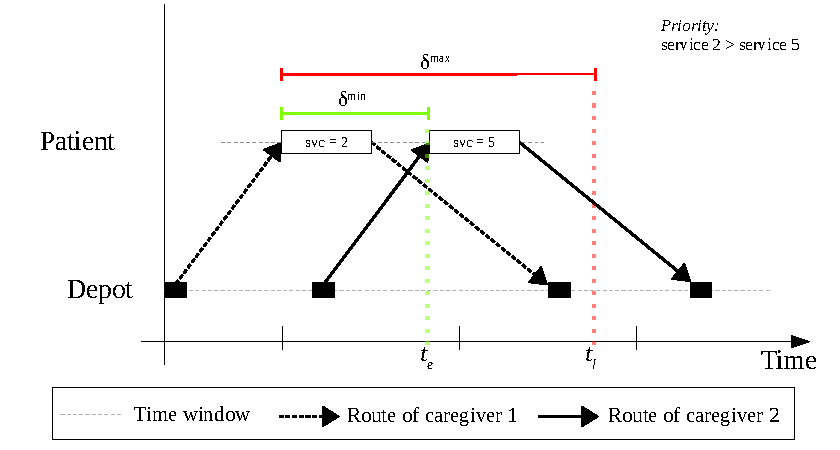
\includegraphics[width=0.8\textwidth,page=1]{fig/sync-tsn2}
   \end{figure}
\end{frame}

\begin{frame}
   \frametitle{The HHCRSP: Own characteristics}
   \textbf{Double service: parallel attendance}
   \begin{itemize}
      \item Services must start simultaneously
   \end{itemize}

   \begin{figure}
      \centering
      \includegraphics[width=0.8\textwidth,page=2]{fig/sync-tsn2}
   \end{figure}
\end{frame}

\begin{frame}
   \frametitle{The HHCRSP: some formal definitions}
   \textbf{Main sets}
   \begin{itemize}
      \item $\mathcal{V}$ : Vehicles/caregivers
      \item $\mathcal{C}$ : Patients/nodes
      \item $\mathcal{S}$ : Service types/skills
   \end{itemize}

\end{frame}

\frame{
   \frametitle{The HHCRSP: some formal definitions}

   \textbf{Objective function}

   \only<1> {
      \begin{gather}
         \mathrm{Minimize~} \lambda_1 D \; +
         \lambda_2 T \; +
         \lambda_3 T^\mathit{max} \nonumber
      \end{gather}
   }

   \only<2-5> {
      \begin{gather}
      \mathrm{Minimize~}\color{InfRed} \lambda_1 \normalcolor D \; +
      \color{green} \lambda_2 \normalcolor T \; +
      \color{blue} \lambda_3 \normalcolor T^\mathit{max} \nonumber
      \end{gather}
   }

   \vspace*{12pt}

   \textbf{Components}
   \begin{itemize}
      \item $D$: Sum of traveled distance
      \item $T$: Sum of tardiness
      \item $T^\mathrm{max}$: Maximum tardiness
   \end{itemize}

   \begin{tikzpicture}[overlay]
      \draw<3>[InfRed,line width=2pt] (4.3,3.4) rectangle +(0.9, 0.7);
      \draw<3>[InfRed,line width=2pt] (-0.4, 1.54) rectangle +(6.4, 0.7);
      \draw<4>[InfRed,line width=2pt] (5.55,3.4) rectangle +(0.9, 0.7);
      \draw<4>[InfRed,line width=2pt] (-0.4, 0.95) rectangle +(6.4, 0.7);
      \draw<5>[InfRed,line width=2pt] (6.85, 3.4) rectangle +(1.3, 0.7);
      \draw<5>[InfRed,line width=2pt] (-0.4, 0.35) rectangle +(6.4, 0.7);
   \end{tikzpicture}
}